\documentclass{beamer}
\usepackage{graphicx}
\usepackage{tikz}
\usepackage{multicol}
\usepackage{listings}
\usepackage{pgfgantt}
\usepackage{xcolor}
\usepackage[utf8]{inputenc}
\setbeamertemplate{footline}[frame number]
\graphicspath{ {./images/} }
\setbeamertemplate{section in toc}[ball unnumbered]

\lstdefinelanguage{yaml}{
  keywords={true,false,null,y,n},
  sensitive=false,
  comment=[l]{\#},
  morecomment=[s]{/*}{*/},
  morestring=[b]',
  morestring=[b]"
}
\lstset{
  basicstyle=\ttfamily\small,
  columns=fullflexible,
  language=yaml,
  breaklines=true,
  frame=single,
  literate={ä}{{\"a}}1 {ö}{{\"o}}1 {ü}{{\"u}}1
           {Ä}{{\"A}}1 {Ö}{{\"O}}1 {Ü}{{\"U}}1
           {ß}{{\ss}}1
}

\lstdefinelanguage{Dockerfile}{
  keywords={FROM, RUN, CMD, LABEL, MAINTAINER, EXPOSE, ENV, ADD, COPY, ENTRYPOINT, VOLUME, USER, WORKDIR, ARG, ONBUILD, STOPSIGNAL, HEALTHCHECK, SHELL},
  sensitive=true,
  morecomment=[l]{\#},
  morestring=[b]",
}
\lstset{
  basicstyle=\ttfamily\small,
  keywordstyle=\color{blue}\bfseries,
  commentstyle=\color{gray},
  stringstyle=\color{orange},
  showstringspaces=false,
  breaklines=true,
  frame=single,
}

\lstdefinelanguage{CSharp}{
  morekeywords={
    abstract, as, base, bool, break, byte, case, catch, char, checked, class, const, continue,
    decimal, default, delegate, do, double, else, enum, event, explicit, extern, false, finally,
    fixed, float, for, foreach, goto, if, implicit, in, int, interface, internal, is, lock, long,
    namespace, new, null, object, operator, out, override, params, private, protected, public,
    readonly, ref, return, sbyte, sealed, short, sizeof, stackalloc, static, string, struct, switch,
    this, throw, true, try, typeof, uint, ulong, unchecked, unsafe, ushort, using, virtual, void,
    volatile, while, var, dynamic, get, set, value, await, async, partial, yield
  },
  sensitive=true,
  morecomment=[l]{//},
  morecomment=[s]{/*}{*/},
  morestring=[b]",
  morestring=[b]',
}

\title{WaterWizards}
\author{Justin Dewitz, Erick Zeiler, Max Kondratov, Julian Ramscheid}
\date{17. Juli 2025}  

\begin{document}

\begin{frame}[plain]
  \titlepage
  \begin{tikzpicture}[remember picture,overlay]
    \node[anchor=south west, xshift=0.2cm, yshift=0.2cm] at (current page.south west) {
\includegraphics[height=2.5cm]{wizblu.png}};
    \node[anchor=south east, xshift=-0.2cm, yshift=0.2cm] at (current page.south east) {
\includegraphics[height=2.5cm]{wizred.png}};
  \end{tikzpicture}
\end{frame}

\begin{frame}
\frametitle{Inhaltsverzeichnis}
\tableofcontents[hideallsubsections] 
\small
\end{frame}

\section{Einleitung}
\begin{frame}
\frametitle{Einleitung}
\begin{itemize}
  \item Was ist WaterWizards?
  \begin{enumerate}
    \item Mulitplayer Real-Time Schiffe versenken
    \item Angriff durch Zauber, die durch Karten repräsentiert werden
    \item Ziel: Zerstörung der gegnerischen Schiffe
  \end{enumerate}
  \item Warum WaterWizards?
  \begin{enumerate}
    \item Schiffe versenken ist ein Klassiker
    \item Durch Real-Time wird es dynamischer
    \item Für jede Altersgruppe interessant
  \end{enumerate}
  \item Was macht WaterWizards besonders?
    \begin{enumerate}
      \item Kombination aus Strategie und schnellen Entscheidungen
      \item Zauber und Karten bringen neue Dynamik ins Spiel
      \item Multiplayer und Echtzeit sorgen für Spannung
    \end{enumerate}
  \item Für wen ist das Spiel gedacht?
    \begin{enumerate}
      \item Strategie-Fans
      \item Familien und Freunde
      \item Alle Altersgruppen
    \end{enumerate}
\end{itemize}
\end{frame}

\section{Organisation}
\begin{frame}
  \frametitle{Organisation}
  \begin{itemize}
    \item git über GitHub für die Versionsverwaltung 
    \item Scrum mit 2-Wochen-Sprints
    \item Kanban/Issue-Board über GitHub
    \item Kommunikation über Discord-Server
  \end{itemize}
\end{frame}

\subsection{Backlog}
\begin{frame}
\frametitle{Backlog}
  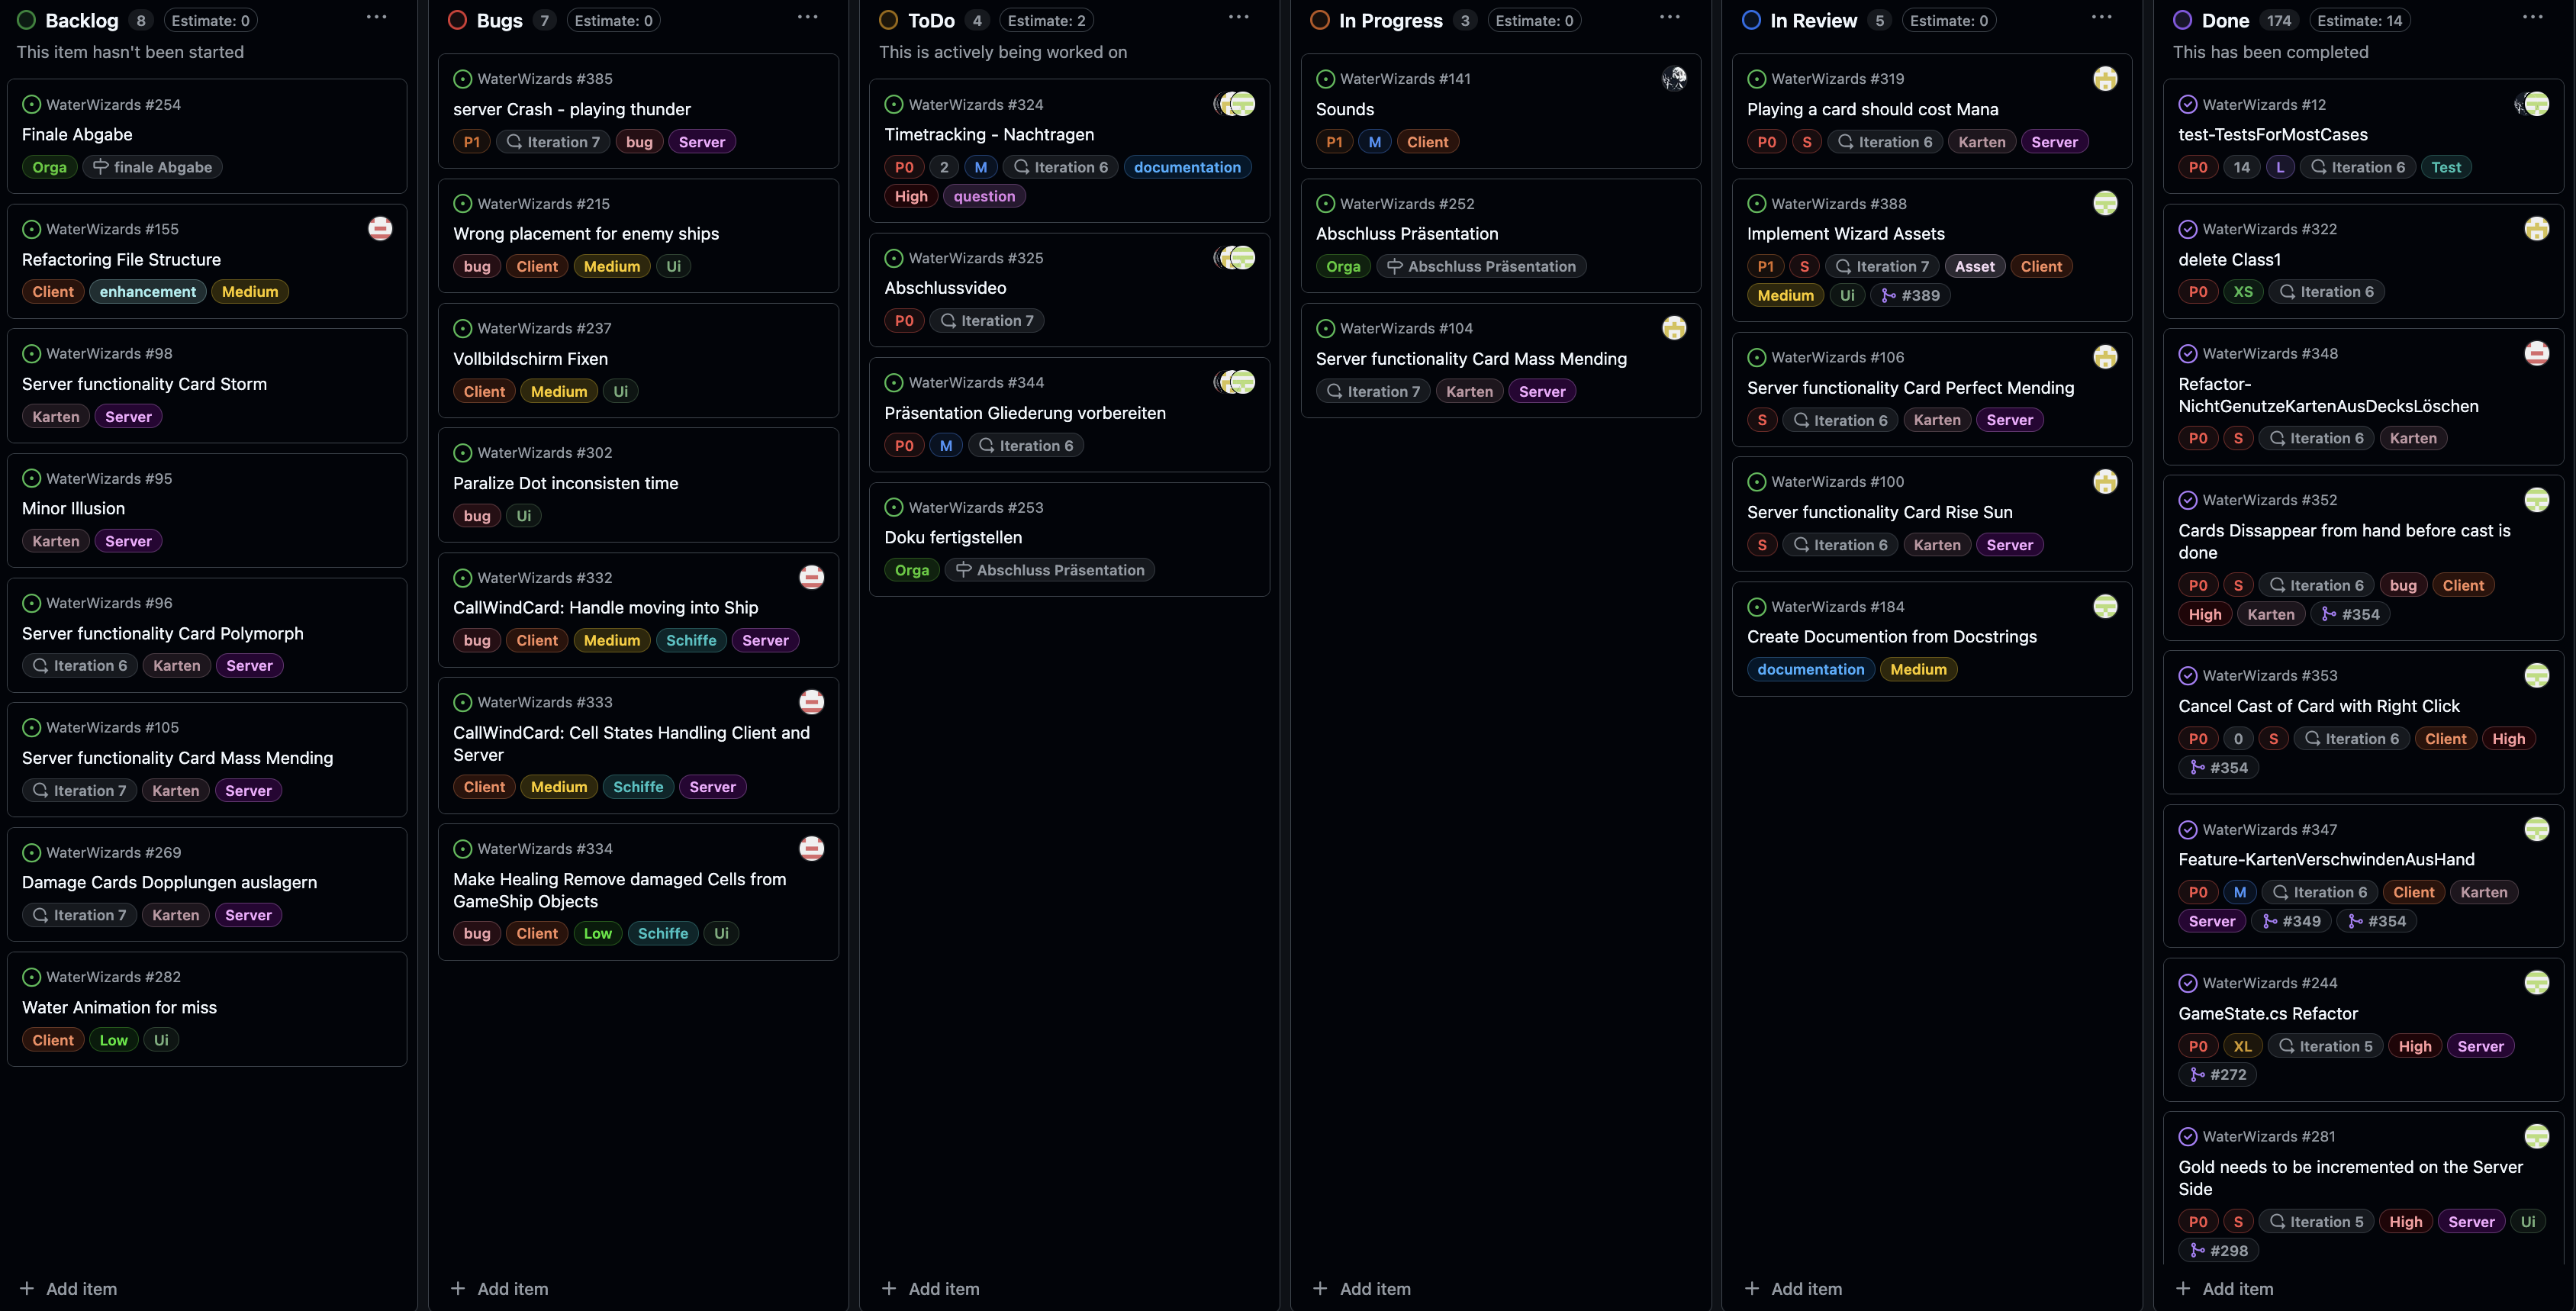
\includegraphics[width=\textwidth]{Kanban.png}
\end{frame}

\subsection{Projektplan}
\begin{frame}
\frametitle{Projektplan}
\begin{center}
\resizebox{\textwidth}{!}{
  \begin{ganttchart}[
    y unit chart=0.3cm,
    vgrid,
    hgrid,
    bar/.append style={fill=blue!40},
    group/.append style={fill=orange!60}, 
    milestone/.append style={fill=red!80},
    group label font=\bfseries\scriptsize,
    bar label font=\scriptsize,
    milestone label font=\scriptsize,
    title label font=\scriptsize
  ]{1}{14}
    \gantttitle{Wochen}{14} \\
    \gantttitlelist{1,...,14}{1} \\

    \ganttgroup{Prototyp}{1}{3} \\
    \ganttbar{Anforderungsanalyse}{1}{1} \\
    \ganttbar{Architektur \& Server Logic}{1}{2} \\
    \ganttbar{UI}{2}{3} \\

    \ganttgroup{Design \& Erste Karten + MVP}{3}{6} \\
    \ganttbar{UI Design}{3}{3} \\
    \ganttbar{Showcase MVP vorbereiten}{4}{6} \\
    \ganttbar{3 Attack Karten}{5}{6} \\

    \ganttgroup{Testen}{5}{12} \\
    \ganttbar{Unit Tests}{5}{11} \\
    \ganttbar{1 Integrationstest}{12}{12} \\

    \ganttgroup{Zielgenaue Implementierung}{5}{10} \\
    \ganttbar{Backend - Frontend Kommunikation verbessern}{5}{8} \\
    \ganttbar{Frontend Feinschliff}{6}{10} \\
    \ganttbar[name=refactoring1]{Refactoring für bessere Lesbarkeit}{7}{9} 
    \ganttbar[inline, bar/.append style={fill=blue!40}]{ }{12}{13} \\
    \ganttgroup{Abschluss}{10}{14} \\
    \ganttbar{Projekt Feinschliff}{10}{14} \\
    \ganttbar{Dokumentation}{13}{13} \\
    \ganttbar{Präsentation}{14}{14} \\
    \ganttmilestone{Projekt Abgabe}{14}
  \end{ganttchart}
}
  \vspace{0.4em}
  {\scriptsize
    \begin{tabular}{@{}ll}
      \textcolor{orange!60}{\rule{0.5em}{0.5em}} & Projektphase (Gruppe) \\
      \textcolor{blue!40}{\rule{0.5em}{0.5em}} & Aufgabe (Task) 
    \end{tabular}
  }
\end{center}
\end{frame}

\subsection{Rollen des Projektes}
\begin{frame}
  \begin{itemize}
    \item Architektur: Justin Dewitz
    \item Dokumentation: Erick Zeiler
    \item Git Repository: Max Kondratov
    \item Koordinator: Julian Ramscheid
    \item Qualitätsmanagement: Paul Schneider (verlassen)
  \end{itemize}
\frametitle{Rollen des Projektes}
\end{frame}

\section{Technologie und DevOps}
\begin{frame}
\frametitle{Technologie und DevOps}
  \begin{itemize}
    \item Programiersprache: C\#
    \item Raylib
    \item LiteNetLib
    \item Nuke für das Build-System
    \item CodeQL für die statische Code-Analyse
    \item GitHub Actions für die CD-Pipeline
    \item GitHub Pages für die Dokumentation
    \item Event-Driven Architektur
    \item Docker für die Containerisierung
    \item Hetzner Server für das Hosting
  \end{itemize}
\end{frame}

\subsection{Raylib}
\begin{frame}
  \frametitle{Raylib}
  \begin{itemize}
    \item Raylib für die grafische Darstellung
    \begin{multicols}{2}
      \begin{itemize}
        \item Leichtgewichtige Library
        \item Einfacher Einstieg
      \end{itemize}
      \columnbreak
      \begin{itemize}
        \item Kein Eigenenes Key- und Maus-Event Handling
      \end{itemize}
    \end{multicols}
    \end{itemize}
\end{frame}

\subsection{LiteNetLib}
\begin{frame}
  LiteNetLib für die Client-Server-Verbindung
  \begin{multicols}{2}
    \begin{itemize}
      \item Einfaches Setup
      \item Einfache Client-Server-Kommunitation über Nachrichten
      \item Einfache Datenübertragung der Spieldaten
    \end{itemize}
    \columnbreak
    \begin{itemize}
      \item Unterstützt nur UDP
    \end{itemize}
  \end{multicols}
\end{frame}


\subsection{DevOps}
\begin{frame}
\frametitle{DevOps}
  \begin{itemize}
    \item CI-Pipeline
    \item CD-Pipeline
    \item Statische Code-Analyse
    \item Pull Requests mit 4-Augen Prinzip
    \item Dokumentation auf Github Pages
  \end{itemize}
\end{frame}

\subsection{CI/CD Pipeline}
\begin{frame}
\frametitle{CI/CD Pipeline}
  \begin{multicols}{2}
    \begin{itemize}
      \item \textbf{CI}
        \begin{itemize}
          \item Nuke build für die Continous-Integration
          \item dotnet \textit{restore, build, test}, werden bei jedem PR ausgeführt
        \end{itemize}
      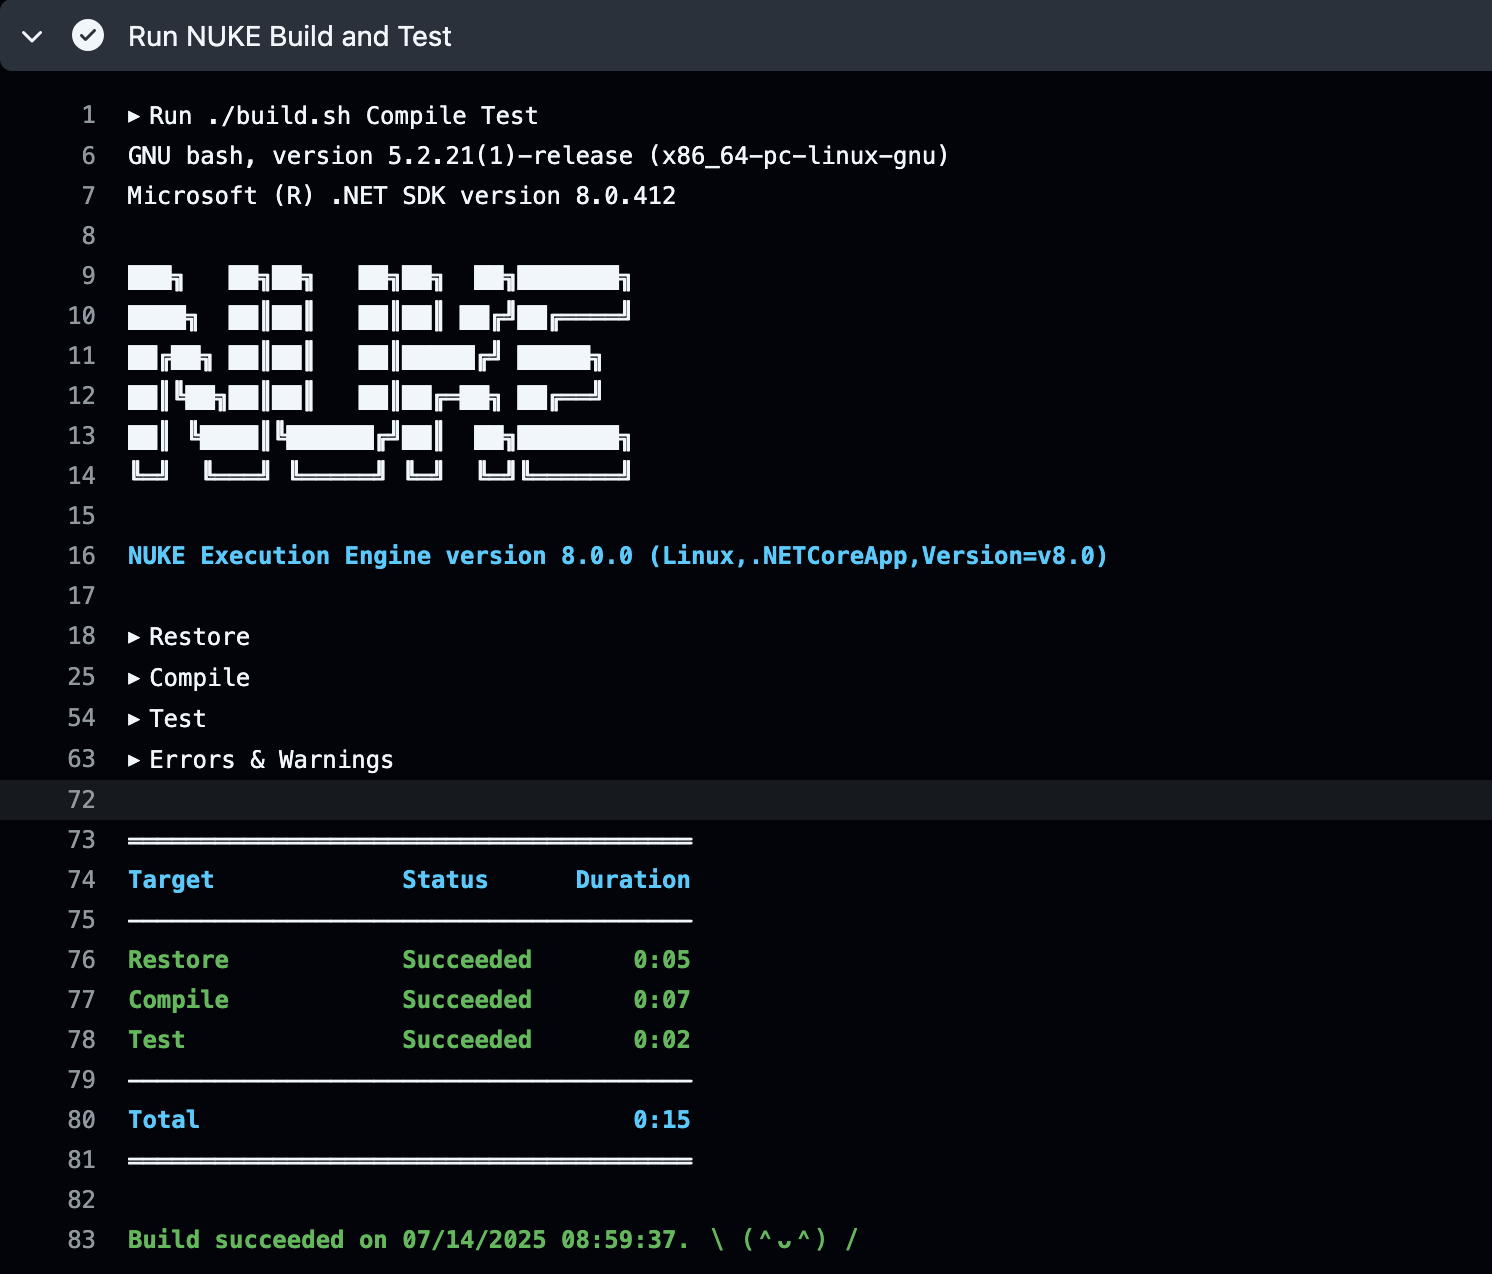
\includegraphics[width=0.4\textwidth]{Nuke-Pipeline.png}
    \end{itemize}
  \columnbreak
    \begin{itemize}
      \item \textbf{CD}
        \begin{itemize}
          \item Github Actions für das Continous-Deployment
          \item Baut eine exe Datei für Windows und eine MacOS App 
        \end{itemize}
        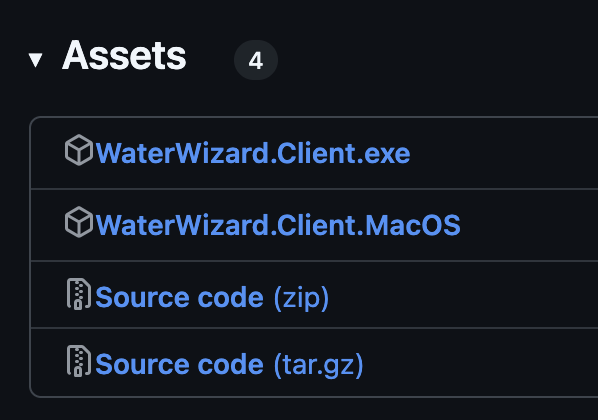
\includegraphics[width=0.4\textwidth]{CD-in-GH.png}
    \end{itemize}
  \end{multicols}
\end{frame}

\subsection{CI-Pipeline Konfiguration}
\begin{frame}[fragile]
\frametitle{CI-Pipeline Konfiguration}
  \begin{lstlisting}[language=yaml, basicstyle=\ttfamily\tiny, breaklines=true]
    name: NUKE Build CI

    on:
      push:
        branches: [ "main", "dev" ] 
      pull_request:
        branches: [ "**" ] 

      workflow_dispatch:

    jobs:
      build:
        runs-on: ubuntu-latest 

        permissions:
          actions: read 
          contents: read 
          security-events: write 

        steps:
          - name: Checkout repository
            uses: actions/checkout@v4
            with:
              fetch-depth: 0 

          - name: Setup .NET SDK
            uses: actions/setup-dotnet@v4
            with:
              dotnet-version: '8.0.x'

          - name: Run NUKE Build and Test
            run: ./build.sh Compile Test
  \end{lstlisting}
\end{frame}

\subsection{CD-Pipeline Konfiguration}
\begin{frame}[fragile]
\frametitle{CD-Pipeline Konfiguration (Teil 1)}
  \begin{lstlisting}[language=yaml, basicstyle=\ttfamily\tiny, breaklines=true]
- name: Publish Client (Windows)
  run: dotnet publish src/WaterWizard.Client/WaterWizard.Client.csproj -c Release -r win-x64 --self-contained true -o ./publish/win --verbosity normal

- name: Publish Server (Windows)
  run: dotnet publish src/WaterWizard.Server/WaterWizard.Server.csproj -c Release -r win-x64 --self-contained true -o ./publish/win-server

- name: Publish Client (MacOS)
  run: dotnet publish src/WaterWizard.Client/WaterWizard.Client.csproj -c Release -r osx-x64 --self-contained true -o ./publish/osx --verbosity normal

- name: Publish Server (MacOS)
  run: dotnet publish src/WaterWizard.Server/WaterWizard.Server.csproj -c Release -r osx-x64 --self-contained true -o ./publish/osx-server

- name: Prepare release assets
  run: |
    mkdir release-assets

    # Find the actual executable names
    WIN_EXE=$(find ./publish/win -name "*.exe" -type f | head -1)
    OSX_EXE=$(find ./publish/osx -type f -executable | grep -v "\.dll$" | grep -v "\.so$" | head -1)
  \end{lstlisting}
\end{frame}

\begin{frame}[fragile]
\frametitle{CD-Pipeline Konfiguration (Teil 2)}
  \begin{lstlisting}[language=yaml, basicstyle=\ttfamily\tiny, breaklines=true]
    if [ -n "$WIN_EXE" ]; then
      cp "$WIN_EXE" release-assets/WaterWizard.Client.exe
    else
      echo "Warning: No Windows executable found"
    fi

    if [ -n "$OSX_EXE" ]; then
      cp "$OSX_EXE" release-assets/WaterWizard.Client.MacOS
    else
      echo "Warning: No MacOS executable found"
    fi

    echo "Release assets:"
    ls -la release-assets/
 
- name: Create GitHub Release & Upload Assets
  uses: softprops/action-gh-release@v2
  with:
    tag_name: ${{ steps.get_version.outputs.tag }}
    name: Release ${{ steps.get_version.outputs.version }}
    body: ${{ steps.changelog.outputs.changelog }}
    draft: false
    prerelease: false
    files: release-assets/*
  env:
    GITHUB_TOKEN: ${{ secrets.GITHUB_TOKEN }} 
  \end{lstlisting}
\end{frame}

\subsection{Statische Code-Analyse}
\begin{frame}
\frametitle{Statische Code-Analyse}
  \begin{itemize}
    \item CodeQL für die statische Code-Analyse
    \item CodeQL eigene Konfigurationsdatei
      \begin{itemize} 
        \item Möglich auch in der CI Kofigurationsdatei
        \item Best Practice getrennt
        \item Simplere Konfiguration durch seperate Datei
      \end{itemize} 
    \item Ergebnisse in GitHub-Security
  \end{itemize}
\end{frame}

\subsection{CodeQL Konfiguration}
\begin{frame}[fragile]
\frametitle{CodeQL Konfiguration (Teil 1)}
  \begin{lstlisting}[language=yaml, basicstyle=\ttfamily\tiny, breaklines=true]
    name: CodeQL

    on:
      push:
        branches: [ main, dev ]
      pull_request:
        branches: [ '**' ]
      workflow_dispatch:

    jobs:
      analyze:
        name: Analyze
        runs-on: ubuntu-latest
        permissions:
          security-events: write
          actions: read
          contents: read

        strategy:
          fail-fast: false
          matrix:
            language: ['csharp']

        steps:
          - name: Checkout repository
            uses: actions/checkout@v4
            with:
              fetch-depth: 0
  \end{lstlisting}
\end{frame}

\begin{frame}[fragile]
\frametitle{CodeQL Konfiguration (Teil 2)}
  \begin{lstlisting}[language=yaml, basicstyle=\ttfamily\tiny, breaklines=true]
      - name: Setup .NET SDK
            uses: actions/setup-dotnet@v4
            with:
              dotnet-version: '8.0.x'

      - name: Initialize CodeQL
        uses: github/codeql-action/init@v3
        with:
          languages: ${{ matrix.language }}
          config-file: .github/codeql/codeql.yml

      - name: Build with NUKE (required by CodeQL)
        run: ./build.sh Compile

      - name: Perform CodeQL Analysis
        uses: github/codeql-action/analyze@v3
        with:
          category: '/language:${{ matrix.language }}'
  \end{lstlisting}
\end{frame}

\subsection{Containerisierung}
\begin{frame}
\frametitle{Containerisierung}
  \begin{itemize}
    \item Docker für die Containerisierung des Servers
    \item Dockerfile im Server-Verzeichnis
    \item Docker Compose im root-Verzeichnis
  \end{itemize}
\end{frame}

\subsection{Dockerfile Code}
\begin{frame}[fragile]
\frametitle{Dockerfile Code}
  \textbf{Dockerfile}
  \begin{lstlisting}[language=Dockerfile,basicstyle=\ttfamily\tiny]
    FROM mcr.microsoft.com/dotnet/sdk:8.0 AS build
    WORKDIR /source

    COPY WaterWizards.sln .

    COPY src/WaterWizard.Server/WaterWizard.Server.csproj ./src/WaterWizard.Server/
    COPY src/WaterWizard.Shared/WaterWizard.Shared.csproj ./src/WaterWizard.Shared/
    COPY src/WaterWizard.Client/WaterWizard.Client.csproj ./src/WaterWizard.Client/
    COPY src/WaterWizardTests/WaterWizardTests.csproj ./src/WaterWizardTests/

    RUN dotnet restore WaterWizards.sln

    COPY src/WaterWizard.Server/ ./src/WaterWizard.Server/
    COPY src/WaterWizard.Shared/ ./src/WaterWizard.Shared/
    COPY src/WaterWizard.Client/ ./src/WaterWizard.Client/
    COPY src/WaterWizardTests/ ./src/WaterWizardTests/

    RUN dotnet publish src/WaterWizard.Server/WaterWizard.Server.csproj -c Release -o /app/publish

    FROM mcr.microsoft.com/dotnet/runtime:8.0 AS final
    WORKDIR /app

    COPY --from=build /app/publish .


    EXPOSE 7777/udp


    ENTRYPOINT ["dotnet", "WaterWizard.Server.dll"]
  \end{lstlisting}
\end{frame}

\subsection{Docker-Compose Code}
\begin{frame}[fragile]
\frametitle{Docker-Compose Code}
  \textbf{docker-compose}
  \begin{lstlisting}[language=yaml,basicstyle=\ttfamily\tiny]
    version: '3.8'

    services:
      waterwizard-server:
        build:
          context: .
          dockerfile: ./src/WaterWizard.Server/Dockerfile
        ports:
          - "7777:7777/udp"
        environment:
          - PUBLIC_ADDRESS=${SERVER_IP}
  \end{lstlisting}
\end{frame}

\subsection{Wiki}
\begin{frame}
\frametitle{Wiki}
  \begin{itemize}
    \item GitHub Wiki für Regeln
      \begin{itemize}
        \item Dokumentation der Projektstruktur
        \item Regeln für Beiträge und Pull Requests
      \end{itemize}
    \item Github Pages für Code-Dokumentation
      \begin{itemize}
        \item Dokumentation erstellt durch Doxygen
      \end{itemize}
    \item ReadME für Projektbeschreibung \& User Dokumentation
      \begin{itemize}
        \item Kurze Einführung ins Projekt
        \item Installation und Nutzung des Spiels
      \end{itemize}
  \end{itemize}  
\end{frame}

\section{Architektur}
\begin{frame}
  \frametitle{Architektur}
  \begin{itemize}
    \item UI/Client
    \item Server/Backend
    \item Shared/Geteilte Klassen
  \end{itemize}
\end{frame}


\subsection{UI/Client - Deckblatt}
\begin{frame}
  \frametitle{UI/Client - Main Menu}
  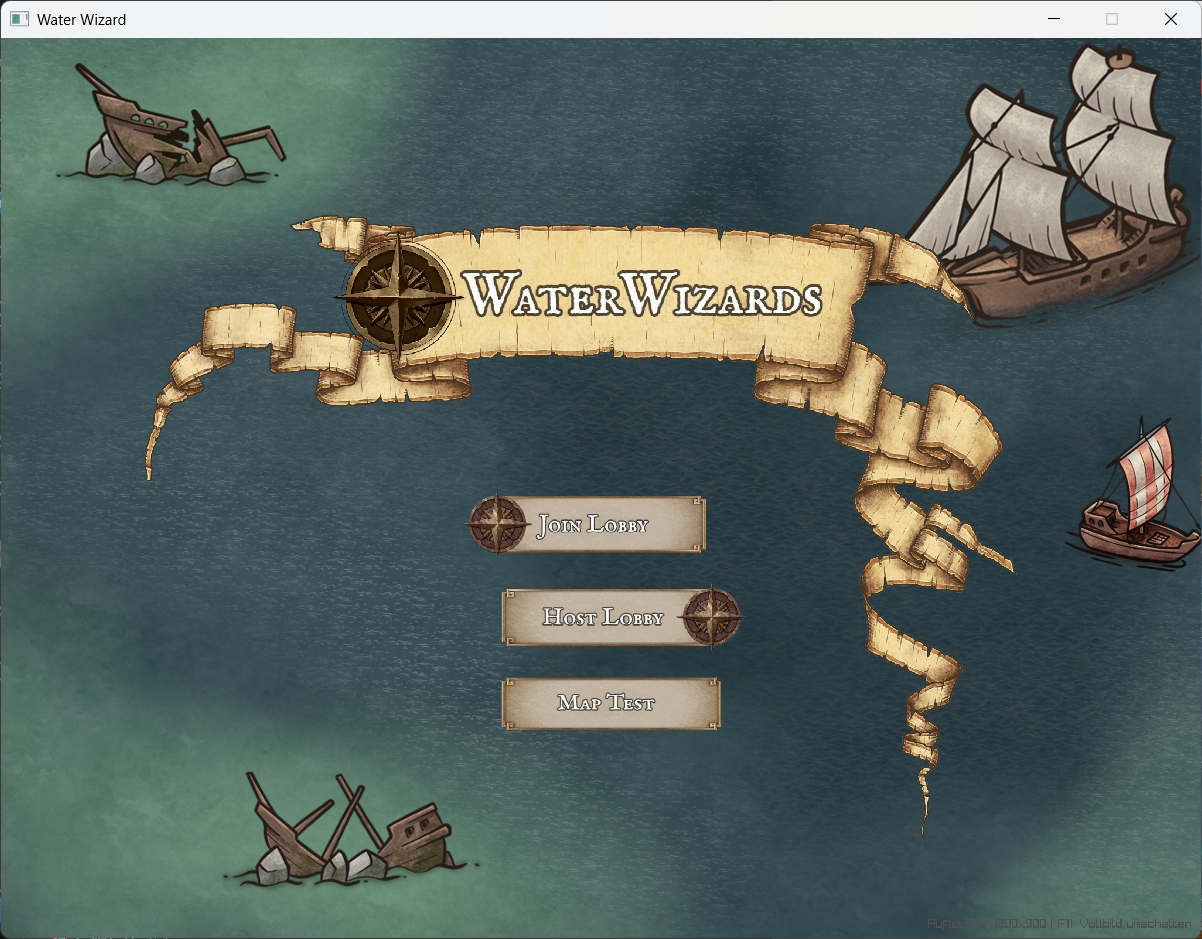
\includegraphics[width=0.95\textwidth]{MainMenuScreen.png}
\end{frame}

\begin{frame}
  \frametitle{UI/Client - Lobby List}
  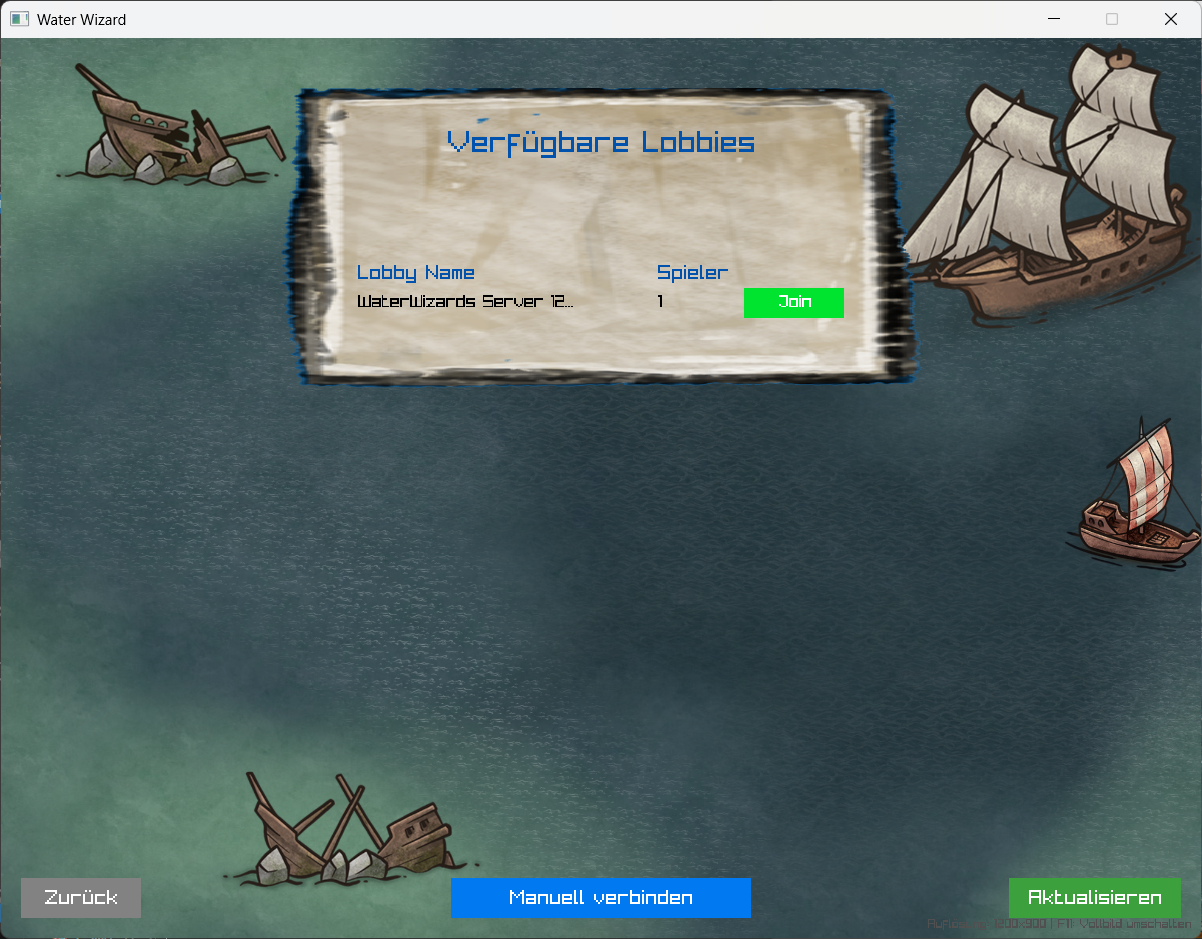
\includegraphics[width=0.95\textwidth]{LobbyListScreen.png}
\end{frame}

\begin{frame}
  \frametitle{UI/Client - Lobby List}
  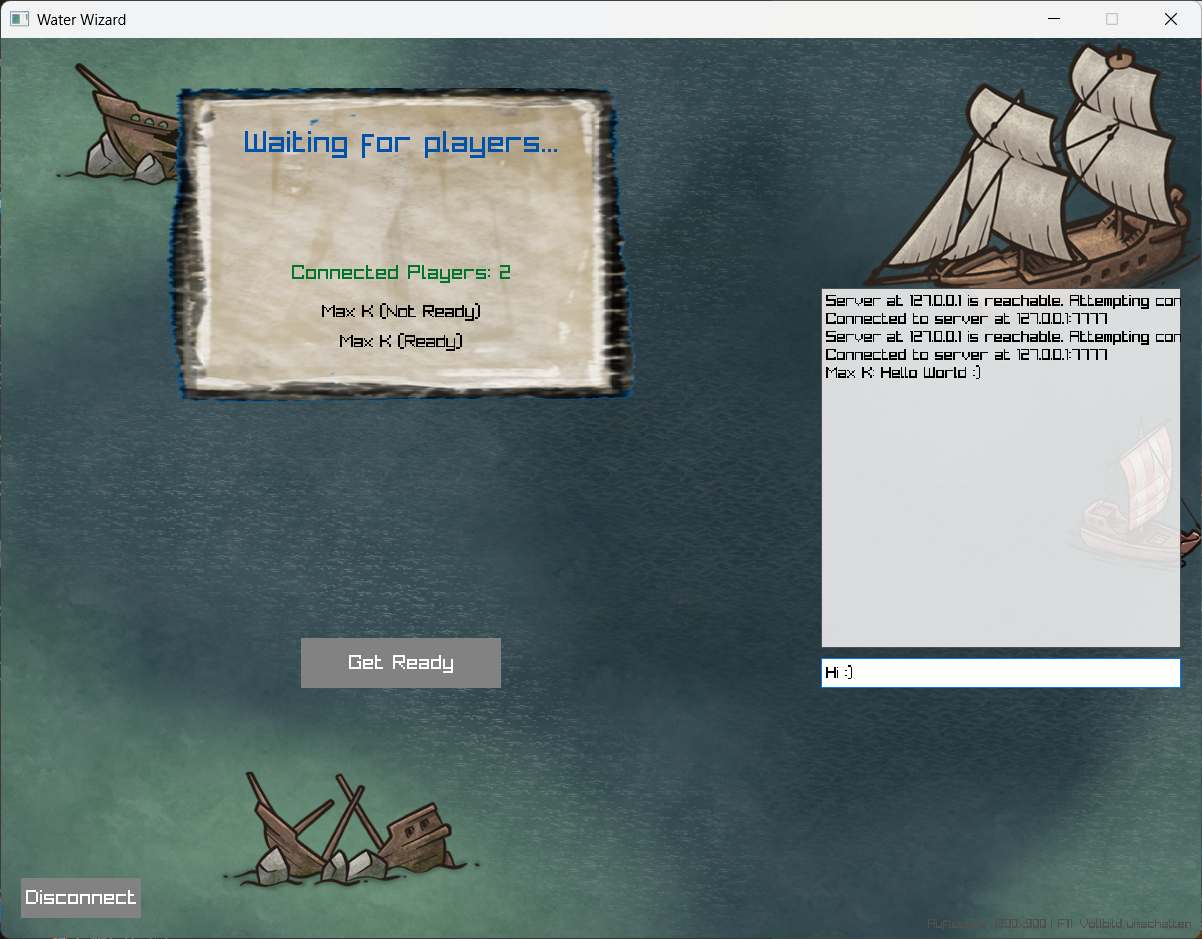
\includegraphics[width=0.95\textwidth]{LobbyScreen.png}
\end{frame}

\begin{frame}
  \frametitle{UI/Client - GameScreen}
  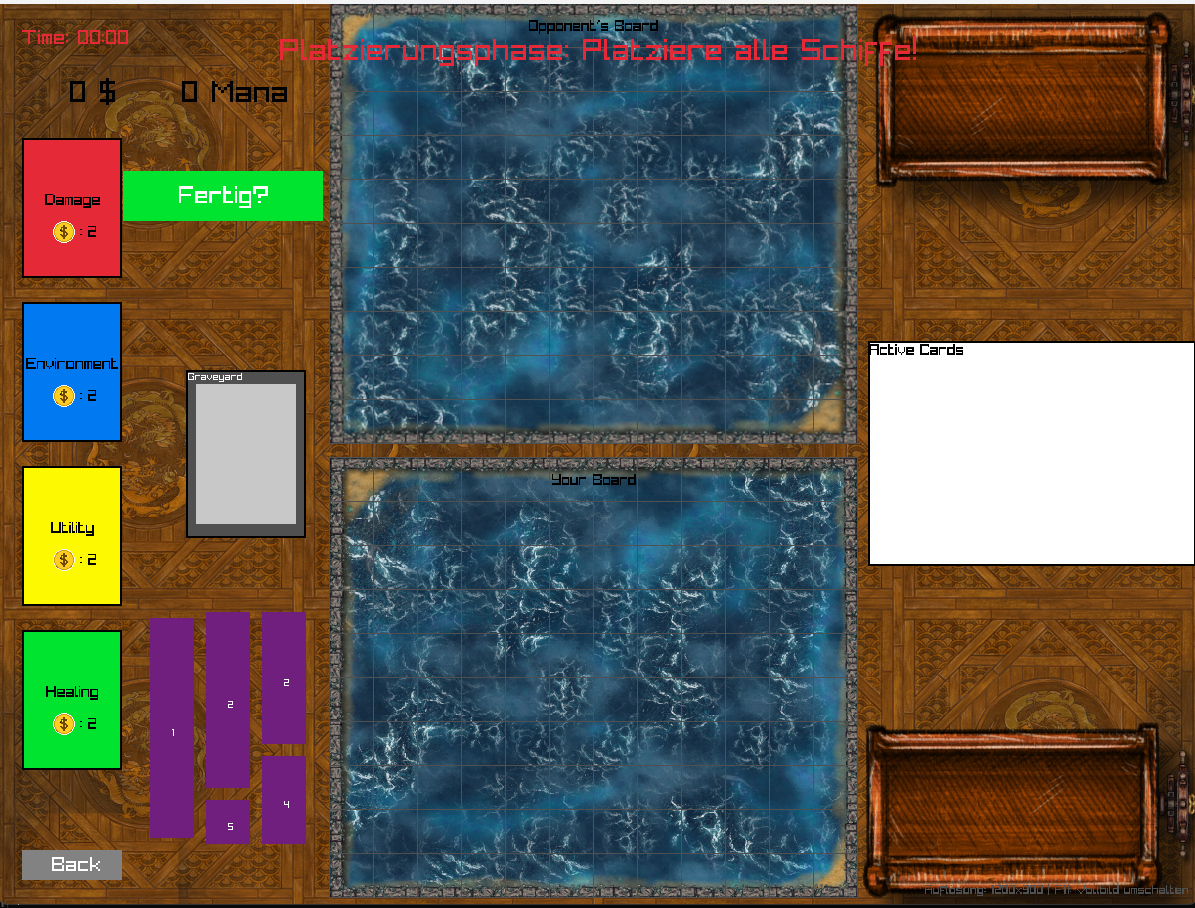
\includegraphics[width=0.95\textwidth]{GameScreen.png}
\end{frame}

\begin{frame}
  \frametitle{UI/Client}
  \begin{itemize}
    \item Grafische Darstellung getrennt von Spielfunktionalität
      \begin{itemize}
        \item Client übernimmt das Anzeigen und Handhabung des User Interfaces 
      \end{itemize}
    \item Interaktive dargestellte Elemente:
    \begin{itemize} 
      \item Das Main Menu, die Kartenstapel, die Schiffe oder die Kartenhand
    \end{itemize}
    \item Rendering und Client-Side Logik werden über Draw-Methoden direkt in der GameLoop ausgeführt wird.
  \end{itemize} 
  \centering
  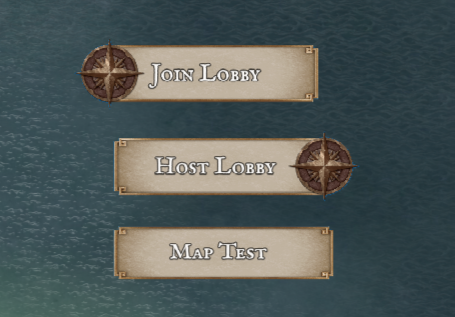
\includegraphics[width=0.55\textwidth]{MainMenuZoomIn.png}
\end{frame}

\subsection{UI-Example}
\begin{frame}[fragile]
  \frametitle{UI-Beispiel aus der MainMenu Klasse}
  \begin{lstlisting}[language=CSharp, basicstyle=\ttfamily\tiny, breaklines=true]
    private static void HandleJoinButton(GameStateManager manager)
    {
        Rectangle joinButton = new(
                    (float)manager.screenWidth / 2 - 140,
                    (float)manager.screenHeight / 2,
                    246,
                    72
                );
        bool hoverJoin = Raylib.CheckCollisionPointRec(Raylib.GetMousePosition(), joinButton);
        if (hoverJoin && Raylib.IsMouseButtonReleased(MouseButton.Left))
        {
            Raylib.PlaySound(SoundManager.ButtonSound);
            manager.SetStateToLobbyList();
        }
        Rectangle textureRec = new(0, 0, joinButtonAsset.Width, joinButtonAsset.Height);
        Raylib.DrawTexturePro(
            joinButtonAsset,
            textureRec,
            joinButton,
            Vector2.Zero,
            0f,
            Color.White
        );
        Raylib.DrawRectangleRec(joinButton, hoverJoin ? new(255, 255, 255, 31) : Color.Blank);
    }
  \end{lstlisting}
\end{frame}

\begin{frame}
  \frametitle{UI Struktur GameScreen}
  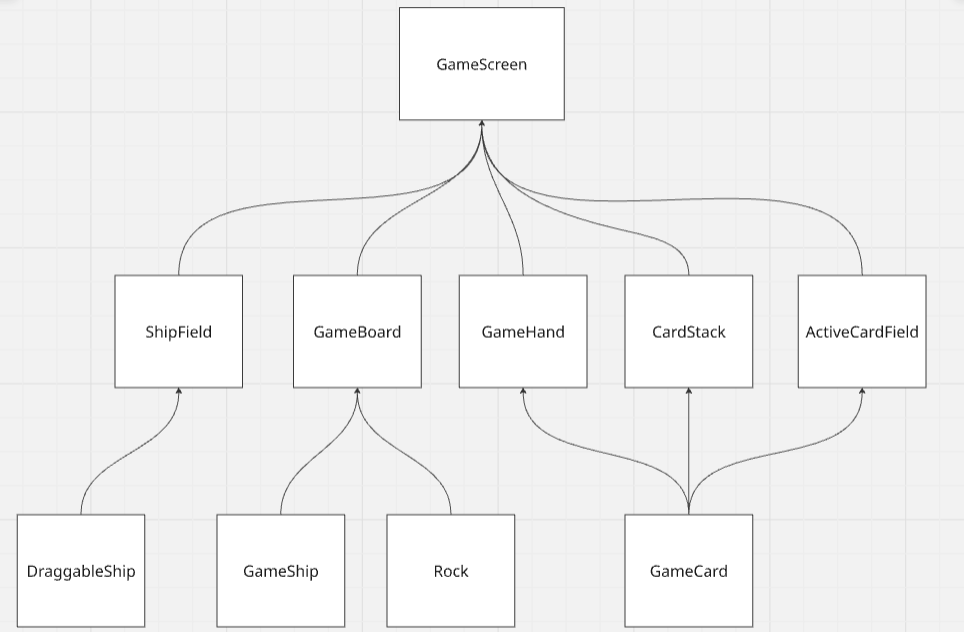
\includegraphics[width=\textwidth]{UI-Struktur.png}
\end{frame}

\subsection{TextureManager}
\begin{frame}[fragile]
\frametitle{TextureManager}
\begin{multicols}{2}
  
  \begin{lstlisting}[language=CSharp, basicstyle=\ttfamily\tiny, breaklines=true]
    public class TextureManager
    {
      private static List<Texture2D> textures = [];
      
      public static Texture2D LoadTexture(string file)
      {
        var texture = Raylib.LoadTexture(file);
        textures.Add(texture);
        return texture;
      }
        
      public static void UnloadAllTextures()
      {
        foreach (var texture in textures)
        {
          Raylib.UnloadTexture(texture);
        }
      }
    }
  \end{lstlisting}
  \columnbreak
  \begin{lstlisting}[language=CSharp, basicstyle=\ttfamily\tiny, breaklines=true]
    public static class SoundManager
    {
    //sounds definition [...]

    public static void LoadSounds()
    {
        CardSound = Raylib.LoadSound("...Sounds/DrawCard.wav");
        ButtonSound = Raylib.LoadSound("...Sounds/ButtonClick.wav");
        //[...]
    }

    public static void UnloadSounds()
    {
        Raylib.UnloadSound(CardSound);
        Raylib.UnloadSound(ButtonSound);
        //[...]
    }
    
    //[...]
  \end{lstlisting}
\end{multicols}
\end{frame}

\subsection{Server/Backend}
\begin{frame}
\frametitle{Server/Backend}
  \begin{itemize}
    \item Das Backend ist in C\# mit der Library LiteNetLib geschrieben
    \item Ein globaler Server der eine Lobby auf Hetzner bereitstellt
    \item Server wird in Docker-Containern ausgeführt
    \item Der Server wird auf dem Port 7777/UDP bereitgestellt
  \end{itemize}
\end{frame}

\subsection{Backend - Client Kommunikation}
\begin{frame}
\frametitle{Backend - Client Kommunikation}
\begin{columns}
  \begin{column}{0.45\textwidth}
    Event-Driven Architektur
    \begin{itemize}
      \item UDP für die Echtzeit-Kommunikation
      \item Nachrichten basiertes Protokoll für beidseitige Kommunikation
    \end{itemize}
  \end{column}
  \begin{column}{0.55\textwidth}
    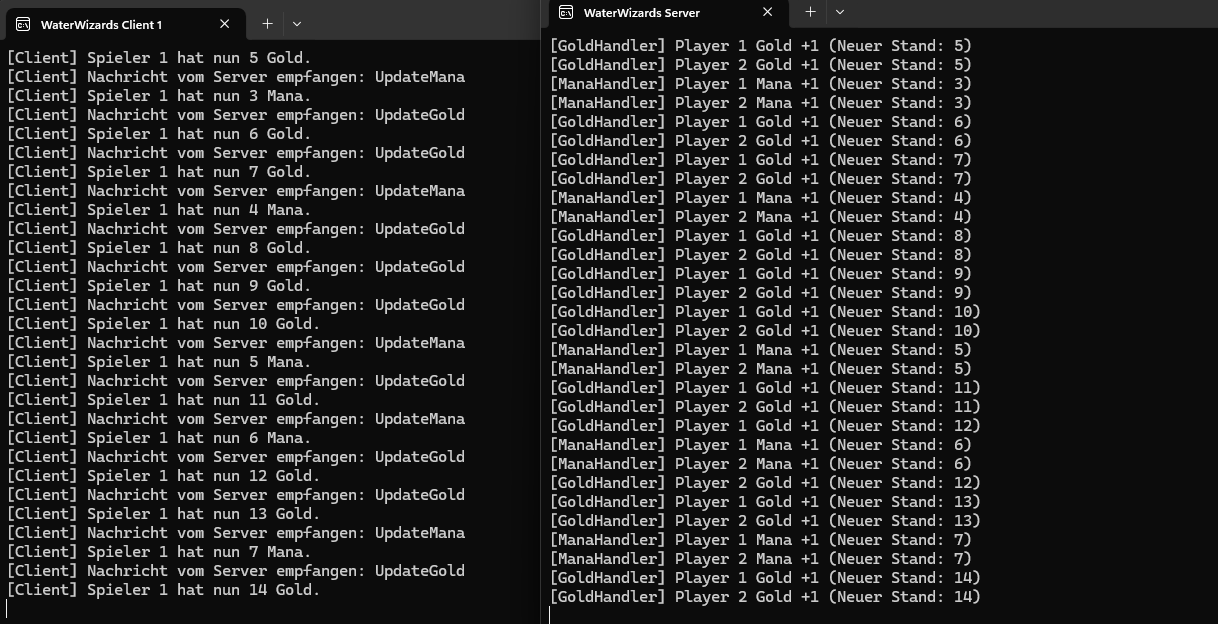
\includegraphics[width=\textwidth]{Server-Client-Logs.png}
  \end{column}
\end{columns}
\end{frame}
\begin{frame}[fragile]
  \begin{column}{0.85\textwidth}
    Basiert auf dem Austausch von Ereignissen (Events)
    \begin{itemize}
      \item Ein Spieler hat eine Karte ausgespielt („CastCard“)
      \item Das Spiel wird pausiert („UpdatePauseState“)
      \item Ein Schiff wurde zerstört („ShipDestroyed“)
      \item Jede Aktion im Spiel löst ein Event aus, das dann an die jeweils betroffenen Clients geschickt wird.
    \end{itemize}
      Der Vorteil: 
      \item
      Das Spiel bleibt reaktionsschnell und alle Spieler sind immer auf dem aktuellen Stand, ohne unnötigen Netzwerkverkehr.

\end{column}
\end{frame}

\subsection{Nachrichtenempfang + Parsing im Client}
\begin{frame}[fragile]
\frametitle{Nachrichtenempfang und Parsing im Client}
  \begin{lstlisting}[language=CSharp, basicstyle=\ttfamily\tiny, breaklines=true]
     private void HandleClientReceiveEvent(
        NetPeer peer,
        NetPacketReader reader,
        byte channelNumber,
        DeliveryMethod deliveryMethod
    )
    {
        try
        {
            string messageType = reader.GetString();
            Console.WriteLine($"[Client] Nachricht vom Server empfangen: {messageType}");

            switch (messageType)
            {
                case "UpdatePauseState":
                    bool isPaused = reader.GetBool();
                    if (isPaused)
                    {
                        GameStateManager.Instance.GetGamePauseManager().PauseGame();
                    }
                    else
                    {
                        GameStateManager.Instance.GetGamePauseManager().ResumeGame();
                    }
                    break;
                case "StartGame":
                    GameStateManager.Instance.SetStateToInGame();
                    break;
                ...
          }
          ...
    }
  \end{lstlisting}
\end{frame}

\subsection{Nachrichten senden an den Server}
\begin{frame}[fragile]
\frametitle{Nachrichten senden an den Server}
  \begin{lstlisting}[language=CSharp, basicstyle=\ttfamily\tiny, breaklines=true]
    public void RequestCardBuy(string cardType)
      {
          if (clientService.client != null && clientService.client.FirstPeer != null)
          {
              var writer = new NetDataWriter();
              writer.Put("BuyCard");
              writer.Put(cardType);
              clientService.client.FirstPeer.Send(writer, DeliveryMethod.ReliableOrdered);
              Console.WriteLine("[Client] Kaufe Karte");
          }
          else
          {
              Console.WriteLine("[Client] Kein Server verbunden, PlaceShip konnte nicht gesendet werden.");
          }
      }
  \end{lstlisting}
\end{frame}
\begin{frame}[fragile]

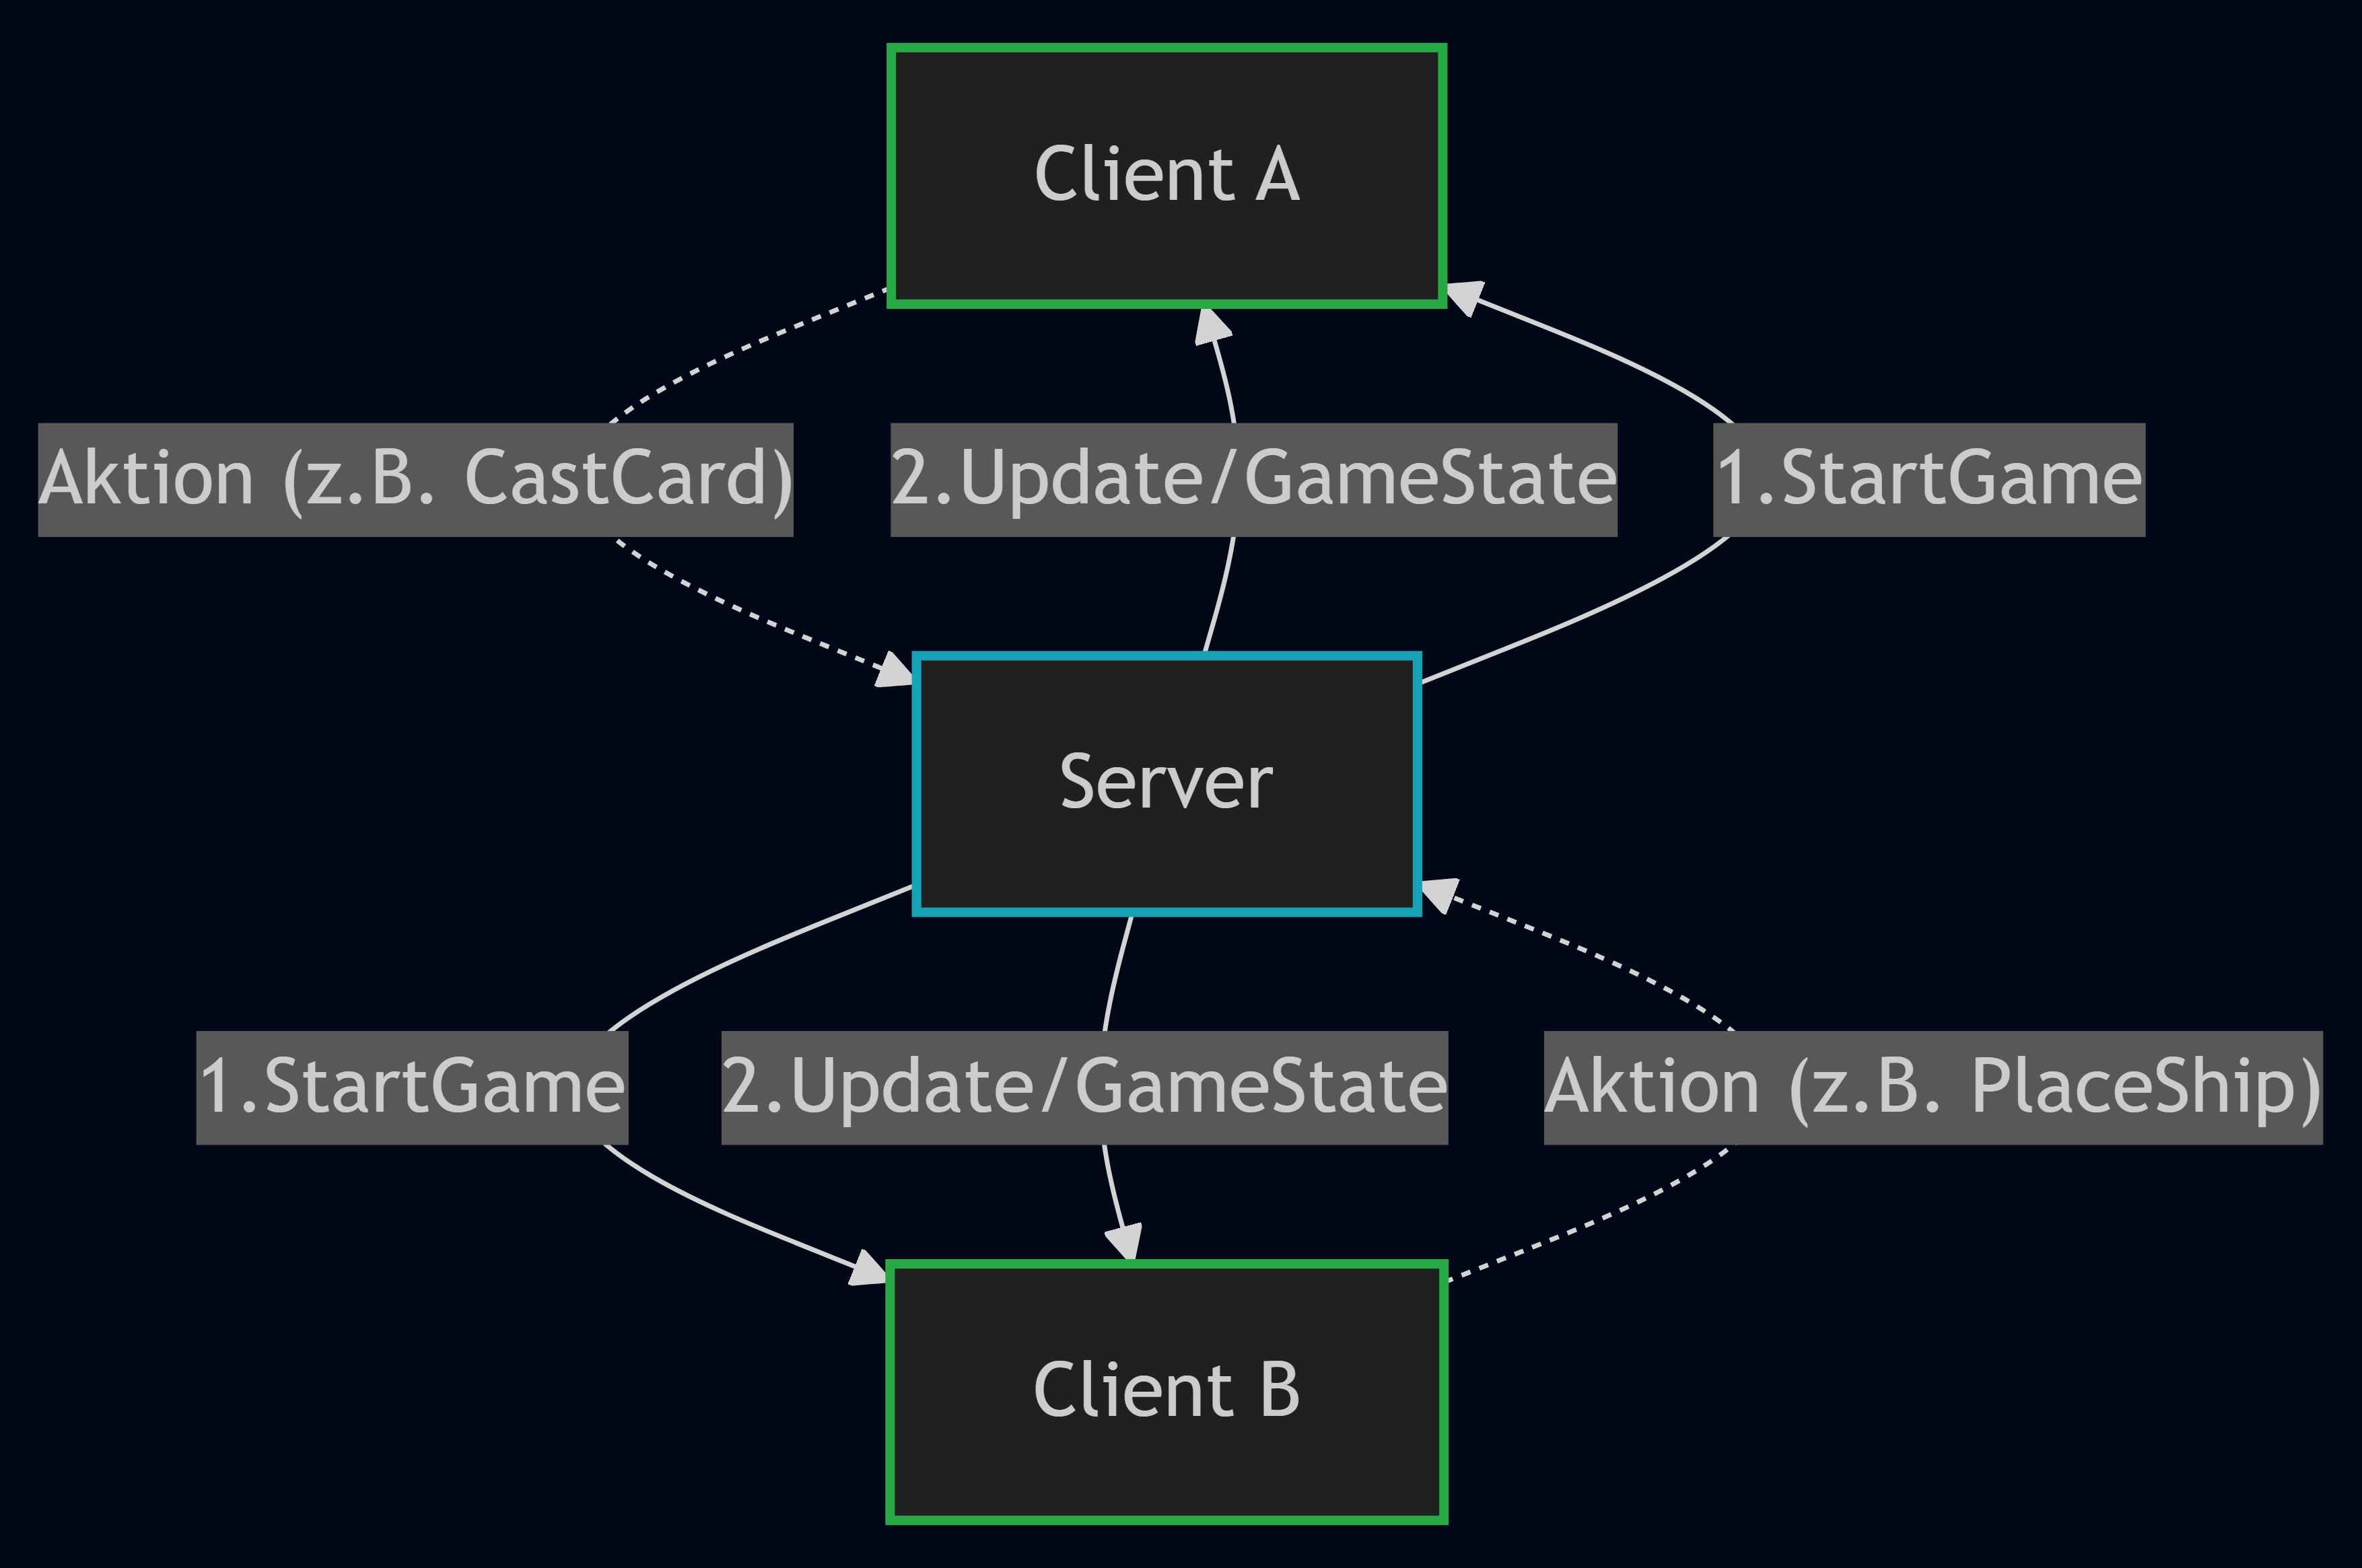
\includegraphics[width=\textwidth]{EDA.png}
\end{frame}

\subsection{GameState}
\begin{frame}[fragile]
  \frametitle{Spielzustand / GameState}
  \begin{itemize}
    \item Programm wird in Zustands-Klassen (States) beschrieben
    \item Spiel wird in der GameState-Klasse beschrieben
    \item Spielinstanzen können getrennt werden
  \end{itemize}
  \textbf{Beispiel: }
  \begin{lstlisting}[language=CSharp, basicstyle=\ttfamily\tiny, breaklines=true]
    public void CheckGameOver()
    {
        foreach (var player in players)
        {
            if (player != null && ShipHandler.AreAllShipsDestroyed(player))
            {
                var winner = players.FirstOrDefault(p => p != player);
                if (winner != null)
                {
                    BroadcastGameOver(winner, player);
                }
            }
        }
    }
  \end{lstlisting}
\end{frame}

\subsection{Factory Pattern}
\begin{frame}[fragile]
\frametitle{Factory Pattern im Backend}
  \begin{itemize}
    \item Das Factory-Pattern wird für die Erstellung von Kartenobjekten verwendet
    \item Für jede Kartenart gibt es eine eigene Factory
  \end{itemize}
  
  \textbf{Beispiel: DamageCardFactory}
  \begin{lstlisting}[language=CSharp, basicstyle=\ttfamily\tiny, breaklines=true]
    public static class DamageCardFactory 
    {
        public static IDamageCard Create(CardVariant variant) 
        {
            return variant switch 
            {
                CardVariant.Firebolt => new FireboltCard(),
                CardVariant.FrostBolt => new FrostBoltCard(),
                CardVariant.Lightning => new LightningCard(),
                _ => throw new ArgumentException($"Unknown variant: {variant}")
            };
        }
    }
  \end{lstlisting}
  
  \textbf{Vorteile:}
  \begin{itemize}
    \item Neue Karten können einfach ergänzt werden
    \item Spiellogik bleibt unverändert
    \item Klare Trennung von Erstellung und Verwendung
  \end{itemize}
\end{frame}

\subsection{Handler}
\begin{frame}[fragile]
\frametitle{Handler}
  \begin{itemize}
    \item Entkoppelt die Logik von der Netzwerkkommunikation
  \end{itemize}
  \textbf{Beispiel: CardHandler}
  \begin{lstlisting}[language=CSharp, basicstyle=\ttfamily\tiny, breaklines=true]
    public void HandleCastCard(Cards card, GameBoard.Point hoveredCoords)
    {
        if (clientService.client != null && clientService.client.FirstPeer != null)
        {
            NetDataWriter writer = new();
            writer.Put("CastCard");
            writer.Put(card.Variant.ToString());
            writer.Put(hoveredCoords.X);
            writer.Put(hoveredCoords.Y);
            clientService.client.FirstPeer.Send(writer, DeliveryMethod.ReliableOrdered);
            Console.WriteLine($"[Client] Karte wirken: {card.Variant} an Position ({hoveredCoords.X}, {hoveredCoords.Y})");
        }
        else
        {
            Console.WriteLine("[Client] Kein Server verbunden, Karte konnte nicht gewirkt werden.");
        }
    }
  \end{lstlisting}
  \textbf{Vorteile:}
  \begin{itemize}
    \item Einfachere Wartbarkeit und Erweiterbarkeit
    \item Einheitliche Handhabung von Aktionen
  \end{itemize} 
\end{frame}

\subsection{Shared}
\begin{frame}
\frametitle{Shared}
  \begin{itemize}
    \item Shared enthält alle Klassen, die sowohl im Client als auch im Server verwendet werden
    \item Definitionen der Karten und der Kartentypen
    \item Definitionen der Schiffe und der Schiffs-Typen
    \item Definition von Mana
  \end{itemize}
\end{frame}

\begin{frame}[fragile]
  \frametitle{Beispiel: Cards}
  \textbf{Definition: }
  \begin{lstlisting}[language=CSharp, basicstyle=\ttfamily\tiny, breaklines=true]
    // Damage Variants
    { CardVariant.MagicAttack, CardType.Damage },
    { CardVariant.ArcaneMissile, CardType.Damage },
    { CardVariant.Firebolt, CardType.Damage },
    { CardVariant.Fireball, CardType.Damage },
    { CardVariant.GreedHit, CardType.Damage },
    { CardVariant.FrostBolt, CardType.Damage },
    { CardVariant.LifeSteal, CardType.Damage },
    //[...]
  \end{lstlisting}
  \textbf{Nutzung: }
  \begin{lstlisting}[language=CSharp, basicstyle=\ttfamily\tiny, breaklines=true]
    public void HandleCast(Cards card, GameBoard.Point hoveredCoords)
    {
        if (clientService.client != null && clientService.client.FirstPeer != null)
        {
            NetDataWriter writer = new();
            writer.Put("CastCard");
            writer.Put(card.Variant.ToString());
            writer.Put(hoveredCoords.X);
            writer.Put(hoveredCoords.Y);
            clientService.client.FirstPeer.Send(writer, DeliveryMethod.ReliableOrdered);
            Console.WriteLine($"[Client] Karte wirken: {card.Variant} an Position ({hoveredCoords.X}, {hoveredCoords.Y})");
        }
        else
        //[...]
    }
  \end{lstlisting}
\end{frame}

\section{Technische Erfahrungen}
\begin{frame}
\frametitle{Technische Erfahrungen}
  \begin{multicols}{2}
    \begin{itemize}
      \item \textbf{Positiv:}
      \item Raylib hat einfachen Einstieg erlaubt
      \item CI/CD Pipeline hat gut Funktioniert
      \item Automatische Validierung CodeQL gut Funktioniert
    \end{itemize}
    \columnbreak
    \begin{itemize}
      \item \textbf{Negativ:}
      \item Server deployment war komplex
      \item Keine CD für den globalen Server
    \end{itemize}
  \end{multicols}
\end{frame}

\section{Analyse}
\begin{frame}
\frametitle{Analyse}

\begin{itemize}
  \item Eigenes Analytics-System zur Auswertung des Repositories
  \item Automatische Ausführung bei jedem Commit, Merge oder Push (Git-Hooks)
  \item Ziel: Transparenz, Codequalität und Team-Insights
\end{itemize}
\end{frame}

\begin{frame}
\frametitle{Was wird analysiert?}
\begin{itemize}
  \item \textbf{Git-Statistiken:} Commits, Branches, letzter Commit, Autor, etc.
  \item \textbf{Code-Statistiken:} Anzahl Dateien, Gesamtzeilen, Codezeilen, Kommentarzeilen, leere Zeilen, Dateitypen, Klassen, Methoden, Interfaces, Properties
  \item \textbf{Entwickler-Statistiken:} Beiträge pro Entwickler, Feature-/Bugfix-/Refactor-/Doku-Commits, Aktivitätsverläufe, Alias-Erkennung
  \item \textbf{Qualitätsmetriken:} Verhältnis Code/Kommentar, Komplexität, Dokumentationsabdeckung, Velocity, aktivster Entwickler, Repository-Alter
\end{itemize}
\end{frame}

\begin{frame}
\frametitle{Beispielhafte Metriken}
\begin{itemize}
  \item \textbf{Code-Komplexität:} z.B. durchschnittliche Methodenlänge
  \item \textbf{Dokumentationsabdeckung:} Anteil dokumentierter Klassen
  \item \textbf{Velocity:} Commits pro Tag im Durchschnitt
  \item \textbf{Aktivster Entwickler:} Name und Beitrag
  \item \textbf{Feature/Bugfix/Refactor-Anteile:} Prozentuale Verteilung der Commits
\end{itemize}
\end{frame}

\begin{frame}[fragile]
\frametitle{Beispiel: Entwickler-Statistiken (JSON-Auszug)}
\begin{lstlisting}[language=json, basicstyle=\ttfamily\tiny, breaklines=true]
{
  "developerStatistics": [
    {
      "name": "Max Mustermann",
      "firstCommit": "2023-01-01T00:00:00Z",
      "lastCommit": "2024-01-15T10:30:00Z",
      "totalCommits": 450,
      "featureCommits": 120,
      "bugFixCommits": 80,
      "refactorCommits": 60,
      "documentationCommits": 40
    }
  ]
}
\end{lstlisting}
\end{frame}
\begin{frame}[fragile]

\frametitle{Beispiel: Entwickler-Statistiken}
\begin{lstlisting}[language=markdown,basicstyle=\ttfamily\tiny,breaklines=true]

##  Developer Statistics
### Erick Zeiler
- **Aliases**: erick, Erick Zeiler, Erickk0
- **Total Commits**: 270
- **First Commit**: 2025-04-23
- **Last Commit**: 2025-07-15
- **Days Active**: 83 days
- **Commit Frequency**: 3.25 commits/day

####  Commit Breakdown
- **Feature Commits**: 100 (37.0%)
- **Bug Fix Commits**: 48 (17.8%)
- **Refactor Commits**: 1 (0.4%)
- **Documentation Commits**: 0 (0.0%)

####  Activity Patterns
- **Average Commits/Week**: 20.8
- **Average Commits/Month**: 67.5
- **Most Active Week**: 2025-W21 (37 commits)
- **Most Active Month**: 2025-05 (101 commits)

\end{lstlisting}

\end{frame}

\begin{frame}
\frametitle{Das Skript: Wie funktioniert unsere Analyse?}
\begin{itemize}
  \item Zentrale Methode \texttt{GenerateRepositoryAnalytics} sammelt alle relevanten Daten:
  \begin{itemize}
    \item Git-Statistiken (Commits, Branches, letzter Commit, Autor, etc.)
    \item Code-Statistiken (Dateien, Zeilen, Klassen, Methoden, Kommentare, etc.)
    \item Entwickler-Statistiken (Beiträge, Aktivität, Aliase)
    \item Qualitätsmetriken (Code-Komplexität, Dokumentationsabdeckung, Velocity)
  \end{itemize}
  \item Die Daten werden automatisch aus dem Repository und dem Quellcode extrahiert – keine manuelle Pflege nötig!
  \item Ergebnisse werden als JSON und Markdown gespeichert und können für Reports oder Visualisierungen genutzt werden.
\end{itemize}
\end{frame}

\begin{frame}[fragile]
\frametitle{Code-Ausschnitt: Analyse-Logik}
\begin{lstlisting}[language=CSharp, basicstyle=\ttfamily\tiny, breaklines=true]
// Git-Statistiken sammeln
var gitCollector = new GitStatisticsCollector(repositoryPath);
analytics.GitStatistics = await gitCollector.CollectAsync();

// Code-Statistiken sammeln
var codeCollector = new CodeStatisticsCollector(repositoryPath);
analytics.CodeStatistics = codeCollector.Collect();

// Entwickler-Statistiken sammeln
var devCollector = new DeveloperStatisticsCollector(repositoryPath);
analytics.DeveloperStatistics = await devCollector.CollectAsync();

// Qualitäts-Metriken berechnen
var metricsCalculator = new QualityMetricsCalculator(analytics);
analytics.QualityMetrics = metricsCalculator.Calculate();
\end{lstlisting}
\end{frame}

\begin{frame}[fragile]
\frametitle{Entwickler-Statistiken (Models/DeveloperStatistics.cs)}
\begin{lstlisting}[language=CSharp, basicstyle=\ttfamily\tiny, breaklines=true]
public class DeveloperStatistics
{
    public string Name { get; set; } = "";
    public DateTime FirstCommit { get; set; }
    public DateTime LastCommit { get; set; }
    public int TotalCommits { get; set; }
    public int FeatureCommits { get; set; }
    public int BugFixCommits { get; set; }
    public int RefactorCommits { get; set; }
    public int DocumentationCommits { get; set; }
    public List<string> CommitMessages { get; set; } = new();
    public List<string> OriginalNames { get; set; } = new();
    public Dictionary<string, int> WeeklyActivity { get; set; } = new();
    public Dictionary<string, int> MonthlyActivity { get; set; } = new();
    // ...
}
\end{lstlisting}

\textbf{Erklärung:}
\begin{itemize}
  \item Für jeden Entwickler werden Commits, Zeiträume, Commit-Arten und Aktivitätsverläufe gespeichert.
  \item So können z.B. die aktivsten Entwickler, Feature-Anteile und Aktivitätsmuster ausgewertet werden.
\end{itemize}
\end{frame}

\begin{frame}[fragile]
\frametitle{Code-Analyse: Zeilenzählung}
\begin{lstlisting}[language=CSharp, basicstyle=\ttfamily\tiny, breaklines=true]
private static FileAnalysis AnalyzeFile(string filePath)
{
    var lines = File.ReadAllLines(filePath);
    var analysis = new FileAnalysis
    {
        FileSize = new FileInfo(filePath).Length,
        TotalLines = lines.Length
    };

    bool inMultiLineComment = false;
    foreach (var line in lines)
    {
        var trimmedLine = line.Trim();
        if (string.IsNullOrEmpty(trimmedLine)) analysis.EmptyLines++;
        else if (trimmedLine.StartsWith("//") || trimmedLine.StartsWith("///")) analysis.CommentLines++;
        else if (trimmedLine.StartsWith("/*")) { analysis.CommentLines++; inMultiLineComment = true; }
        else if (trimmedLine.Contains("*/")) { analysis.CommentLines++; inMultiLineComment = false; }
        else if (inMultiLineComment) analysis.CommentLines++;
        else analysis.CodeLines++;
    }
    return analysis;
}
\end{lstlisting}

\textbf{Erklärung:}
{\footnotesize
\begin{itemize}
  \item Jede Datei wird zeilenweise analysiert.
  \item Es wird unterschieden zwischen Codezeilen, Kommentarzeilen und leeren Zeilen.
  \item Auch mehrzeilige Kommentare werden korrekt erkannt.
\end{itemize}
}
\end{frame}

\begin{frame}
\frametitle{Nutzen für das Team}
\begin{itemize}
  \item Transparenz über Beiträge und Teamaktivität
  \item Motivation durch sichtbare Fortschritte und Statistiken
  \item Grundlage für gezielte Verbesserungen im Entwicklungsprozess
\end{itemize}
\end{frame}

\section{Erfahrungen und Fazit}
\begin{frame}
\frametitle{Erfahrungen und Fazit}
\begin{itemize}
  \item Team Mitglied hat das Team verlassen.
  \item Seine Arbeit konnte übernommen werden.
  \item Gesamte Arbeitslast ist gestiegen. 
\end{itemize}
\end{frame}


\end{document}